\documentclass{standalone}

\usepackage{tikz}
\usetikzlibrary{automata, arrows.meta, positioning, shapes}

\begin{document}
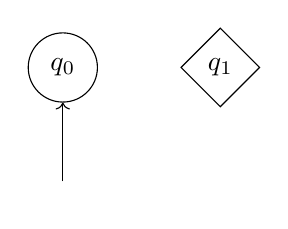
\begin{tikzpicture} [node distance = 2 cm, on grid]
  \node (q0) [state,
  initial below,
  initial distance=1cm,
  initial text={}] {$q_{0}$};

  \node (q1) [state,
  initial by diamond,
  right = of q0] {$q_{1}$};
\end{tikzpicture}
\end{document}
